\documentclass[12pt]{article}

% Math package
% leqno means numbered equations are displayed with the numbers to the left of
% the equations instead of to the right ("left equation numbers")
\usepackage[leqno]{amsmath}

% Geometry package for setting margins
\usepackage{geometry}
% Set margins
\geometry{margin=1in}

% Color package for highlighting text and array columns
\usepackage[table]{xcolor}

% Command \T now inserts a bold math t (for convenience)
\newcommand{\T}{\mathbf{t}}
% Command \F now inserts a bold math f (for convenience)
\newcommand{\F}{\mathbf{f}}

% Package for sans-serif font
\usepackage{helvet}
\renewcommand{\familydefault}{\sfdefault}

% Package for the Aboxed command
\usepackage{mathtools}

% Package for creating equations side-by-side
\usepackage{multicol}

% Package for adding space between paragraphs
\usepackage[skip=10pt plus1pt, indent=20pt]{parskip}

% Package for changing enumerate letters
\usepackage{enumitem}

% Adding "Page {number} of {total}" in footer
\usepackage{lastpage}
\usepackage{fancyhdr}
\fancyfoot[C]{
    Page
    \thepage\
    of
    {\hypersetup{linkcolor=black}\pageref{LastPage}}
}
\pagestyle{fancy}
% Remove horizontal line from header
\renewcommand{\headrulewidth}{0pt}

% I'm more used to typing \infin for infinity symbol :P
\newcommand*{\infin}{\infty}

% Colors
\usepackage{xcolor}
\definecolor{codegreen}{rgb}{0,0.6,0}
\definecolor{codegray}{rgb}{0.5,0.5,0.5}
\definecolor{codepurple}{rgb}{0.58,0,0.82}
\definecolor{backcolour}{rgb}{0.92,0.92,0.92}
\definecolor{rulecolour}{rgb}{0.5,0.5,0.5}

% For code blocks
\usepackage{listings}
\lstdefinestyle{mystyle}{
    backgroundcolor=\color{backcolour},
    commentstyle=\color{codegreen},
    keywordstyle=\color{magenta},
    numberstyle=\tiny\color{black},
    stringstyle=\color{codepurple},
    basicstyle=\ttfamily\footnotesize,
    rulecolor=\color{black},
    breakatwhitespace=false,
    breaklines=true,
    captionpos=b,
    keepspaces=true,
    numbers=left,
    numbersep=5pt,
    showspaces=false,
    showstringspaces=false,
    showtabs=false,
    tabsize=2
}
\lstset{style=mystyle}

% Package for diagonal fractions
\usepackage{xfrac}

% Floating images
\usepackage{float}

% Package for making the "Figure #:" bold in figure captions
\usepackage{caption}
\captionsetup{labelfont=bf}

% Hyperlinks
\usepackage{hyperref}
\hypersetup{
    colorlinks,
    citecolor=black,
    filecolor=black,
    linkcolor=black,
    urlcolor=black
}

% Package for table of contents
\usepackage{tocloft}
% Fill table of contents lines with dots
\renewcommand{\cftsecleader}{\cftdotfill{\cftdotsep}}
% --- Setting the spacing between lines in table of contents ---
% Spacing after section
\renewcommand\cftsecafterpnum{\vskip15pt}
% Spacing after subsection
\renewcommand\cftsubsecafterpnum{\vskip15pt}
% Spacing after subsubsection
\renewcommand\cftsubsubsecafterpnum{\vskip15pt}

% Appendix package
\usepackage[title, titletoc]{appendix}

% Shortcut command for making a link with the link as the text
\newcommand*{\urllink}[1]{\href{#1}{#1}}

% Shortcut command for "Figure #"
\newcommand*{\fig}[1]{\hyperref[fig:#1]{Figure~\ref{fig:#1}}}

\bibliographystyle{ieeetr}

\begin{document}

    % ----- Title page -----
    \newgeometry{left=1.3in, right=1.3in}
\newlength\myheight
\newlength\mydepth
\settototalheight\myheight{Xygp}
\settodepth\mydepth{Xygp}
\setlength\fboxsep{0pt}
\setlength{\fboxrule}{0pt}
\begin{titlepage}
    \Huge\noindent\textbf{EECS 3221 Report}

    \Large\noindent\textbf{A Comparison of Real Time Operating Systems and the Linux Operating System}

    \Large\noindent Daniel Di Giovanni --- 218204818

    \large\noindent\today

    \vfill

    \normalsize
    \begin{center}
        \rule{\textwidth}{1pt}\\
    \end{center}

    \noindent\textbf{My signature below attests that this submission is my original work:}
        % Make sure this line is justified
        \unskip\parfillskip 0pt \par

    \small\noindent
        Following professional engineering practice, I bear the burden of
            proof for original work. I have read the
            \href
                {https://www.yorku.ca/secretariat/policies/policies/academic-honesty-senate-policy-on/}
                {\color
                    {red}
                    {York University Senate Policy on Academic Integrity}
                }
            and the
            \href
                {http://www.cse.yorku.ca/admin/coscOnAcadHonesty.html}
                {\color
                    {red}
                    {EECS Academic Honesty Guidelines}
                }
            and confirm that this work is in accordance with the Policy.
    \vspace*{0.5cm}
    \noindent

    \begin{center}
        \begin{tabular}{ll}
            \raisebox{-30pt}{\fbox{
\includegraphics[height=30pt]{images/singature.jpeg}}} & \raisebox{-30pt}{\fbox{\today}}\\
            \makebox[2.5in]{\hrulefill} & \makebox[2.5in]{\hrulefill}\\
            \textbf{Signature} & \textbf{Date}\\
        \end{tabular}
    \end{center}
\end{titlepage}
\restoregeometry


    % Numbering i, ii, iii, ...
    \pagenumbering{roman}

    % ----- Table of contents -----
    {\hypersetup{linkcolor=black}
    \tableofcontents
    \thispagestyle{plain}
}


    % Number 1, 2, 3, ...
    \pagenumbering{arabic}

    % Remove header text
    \markboth{}{}

    % ===== Sections =====

    % ----- Introduction -----
    \section{Introduction and Background}
% \section*{Introduction and Background}
% \addcontentsline{toc}{section}{Introduction and Background}
% Remove header text
\markboth{}{}
    An operating system is a computing layer that separates the hardware of the
        computer from the programs that run on it.
    It provides the \textit{environment} for other programs to do useful work
        \cite[p. 4]{textbook}.
    The fundamental tasks of an operating system include allocating resources
        (such as memory and CPU time), handling the control of input/output
        (I/O) devices, and ensuring proper usage of the computer and preventing
        errors \cite[pp. 3-5]{textbook}.

    The most important part of an operating system is the \textit{kernel}. It is
        the first program loaded into memory on startup and is the one program
        that is always running on the computer \cite[pp. 6-7, 22]{textbook}.
    Along with the kernel, operating systems also include
        \textit{middleware frameworks} that ease application development, and
        \textit{system programs} that help the system run but are not part of
        the ever-running kernel.
    All of this supports the execution of \textit{application programs}, which
        are the programs that provide functionality to the end user
        \cite[p. 4, 7]{textbook}.
    A diagram of system organization with the kernel is shown in
        \fig{kernel_in_os}.

    \begin{figure}[H]
        \centering
        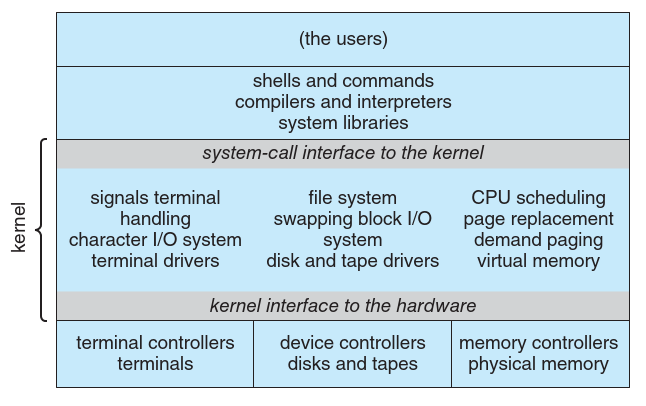
\includegraphics
            [width=0.7\textwidth]
            {images/kernel_in_os.png}
        \caption
            [Diagram of a kernel within the operating system]
            {Diagram of a kernel within the operating system \cite[p. 82]{textbook}.}
        \label{fig:kernel_in_os}
    \end{figure}

    In industrial and commercial computing applications, the choice of an
        operating system is crucial.
    It affects the performance, security, and maintainability of the system.
    As an example, consider the secure boot of an embedded system.
    Secure boot, an important security technique to ensure that the kernel code
        has not been modified, is often neglected in embedded systems.
    The absence of secure boot allows the system to boot faster with less memory
        and energy consumption---at the cost of leaving the boot process and
        internal software vulnerable.
    However, it was discovered that the introduction of secure boot software
        caused boot-up time to increase by only 4\%, whereas a hardware
        implementation of secure boot caused a 36\% increase
        \cite[pp. 11-12]{ingelhag}.
    Clearly, the operating system has a significant impact on the overall
        quality of the system.

    Two important classes of operating systems/kernels will be discussed
        here: the Linux operating system and real-time operating systems (RTOSs).
    The Linux kernel is a free and open source implementation of an operating
        system kernel.
    It is used ubiquitously not only for desktop computers, but also for servers
        and embedded devices with a broad range of commercial and
        industrial applications \cite{whatislinux}.
    The Linux kernel is a tried-and-tested system with high flexibility and
        extendability.
    RTOSs are more vague, being defined not by a specific implementation, but by
        the ability to manage systems with complex time and resource
        constraints \cite{rtos-overview}.
    RTOSs need to be able to meet strict deadlines associated with external
        events using limited resources.
    In short, ``a real-time system is one whose correctness involves both the
        logical correctness of the outputs and their timeliness''
        \cite{laplante}.

    The objective of this report is to provide a thorough comparison of the
        Linux operating system/kernel with RTOS/real-time kernels to aid in the
        decision of which operating system to use.


    \section*{Overview of Linux}
\addcontentsline{toc}{section}{Overview of Linux}
    When ``Linux'' is referred to, an entire operating system is often being
        referenced.
    However, ``Linux'' is just the kernel.
    The Linux kernel is used in combination with other software to make a
    complete operating system.
    The entire operating system (with the Linux kernel inside) is called a
        ``Linux distribution'' (for example, Ubuntu and Debian for PCs)
        \cite{stallman}.
    The ability to extend and modify a Linux operating system is where its
        flexibility originates.

    Since Linux is an open source kernel, anyone can read, use, and modify the
        code.
    And since it is just a kernel, it \textit{requires} additional software to
        be useful.
    This leads to a wide variety of adaptations of the Linux-based operating
        systems to fit many different needs \cite{comparative-os}.

    Many Linux distributions are desktop-focused, creating an easy
        user-interface, similar to Microsoft's Windows and Apple's MacOS, with
        the ability to run virtually all of the programs expected from a desktop
        computer.
    Linux operating systems are also a popular choice for web servers and have
        become the backbone of enterprise computing \cite{grandview}.
    According to the Linux Foundation, Linux powers the majority of the public
        cloud \cite{linux-public-cloud}, and some companies, like Amazon Web
        Services, have developed their own Linux distribution for use in their
        products \cite{aws-linux}.

    Most pertinent to this report, however, is the use of Linux in embedded
        applications.
    While some embedded devices do not employ an operating system (these are
        called \textit{bare-metal} systems, and they forgo an operating system
        to conserve resources \cite{bare-metal}), most are complex enough to
        require an operating system.
    And when an embedded system requires an operating system, Linux is an
        appropriate choice for its kernel.

    The Linux Foundation estimates that 62\% of embedded systems use a
        Linux-based operating system \cite{linux-public-cloud}.
    This is possible because of the high degree of modularity within the Linux
        kernel, making it easy to configure the kernel to specific hardware
        \cite{embedded-textbook}.
    Further, developers of embedded Linux distributions have the ability to
        exclude packages specific to desktops, like user systems and GUI
        environments, opting instead for packages suited for embedded development,
        like cross-development tools, different types of drivers, and debugging
        and profiling tools \cite{embedded-textbook}.
    This extensibility and flexibility makes embedded Linux a great choice.


    \section*{Overview of Real-Time Operating Systems}
\addcontentsline{toc}{section}{Overview of Real-Time Operating Systems}
    Real-time systems are systems with rigid timing requirements
        \cite[pp. 46]{textbook}.
    RTOSs can be used to provide a layer of abstraction between the software
        handling real-time events and the underlying hardware.
    These operating systems must be high-performance with predictable and
        deterministic behavior \cite{rtos-definition}.

    Real-time systems can be categorized into \textit{soft} and \textit{hard}
        systems.
    According to Intel, hard real-time systems refer to systems where missing a
        deadline means failure of the system \cite{intel-hard-soft-real-time}.
    In soft real-time systems, however, the focus in on optimizing quality of
        service.
    Missing a deadline would result lower-quality service, not in a system
        failure \cite{hard-soft-real-time}.
    As an example, a robotic arm needs to be instructed to stop \textit{before}
        it hits a wall, and failure to meet this deadline will cause the arm to
        break.
    This means the robotic arm is a hard real-time system
        \cite[pp. 45-46]{textbook}.
    A consumer smartphone would be a soft real-time system because while a
        lagging phone is frustrating to the user, it is not catastrophic.

    There are many strategies for implementing a RTOS.
    The focus is on responding to external (real-time) events in a time period
        that is minimal and predictable.
    The time taken to respond to an event is called \textit{dispatch latency}.
    As shown in \fig{rtos_dispatch_latency}, dispatch latency consists of many
        aspects, like interrupt processing, preempting and managing conflicts
        with other processes, and executing the actual process.
    Thus, the operating system's process scheduling algorithm is of utmost
        importance.

    \begin{figure}[H]
        \centering
        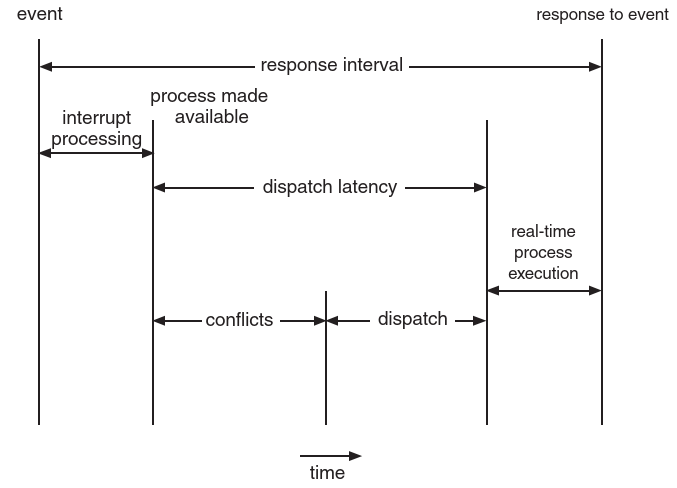
\includegraphics
            [width=0.7\textwidth]
            {images/rtos_dispatch_latency.png}
        \caption
            [Dispatch latency of an event]
            {Dispatch latency of an event \cite[p. 229]{textbook}.}
        \label{fig:rtos_dispatch_latency}
    \end{figure}

    To meet strict deadline requirements, a priority-based scheduler is
        necessary.
    Such a scheduler enables higher-priority processes to preempt lower-priority
        ones \cite[p. 229]{textbook}.
    For hard real-time systems, both the CPU burst time of the process and its
        deadline must be known.
    When a process is ready to execute, the scheduler can decide whether or not
        it is possible to meet the process's deadline, and choose to schedule it
        accordingly.
    This is called an \textit{admission-control algorithm}
        \cite[pp. 229-230]{textbook}.

    \textit{Rate-monotonic} scheduling can be used to schedule periodic real-time tasks.
    In this algorithm, processes with shorter periods are assigned higher
        priorities, since they have a shorter deadline.
    For this type of scheduling to work its CPU burst time must be the same
        every time it executes, and must be shorter than its deadline and
        period.
    A pitfall of rate-monotonic scheduling is that it is not always able
        schedule processes even if there is enough CPU time for them
        \cite[pp. 230-232]{textbook}.

    Another real-time scheduling technique is called
        \textit{earliest-deadline-first (EDF)}.
    In this algorithm, higher priority is given to processes whose deadline is
        sooner.
    This way, a process near its deadline can preempt a process that has more
        time to spare.
    EDF scheduling can achieve a CPU usage near 100\%, thus being able to
        schedule more processes than rate-monotonic scheduling
        \cite[pp. 232-233]{textbook}.

    Implementing an RTOSs is more complex than using a Linux-based operating
        system, but the complexity is the cost for performance.
    For hard real-time systems, an RTOS is necessary to meet performance
        requirements.
    For soft real-time systems, tradeoffs must be balanced to determine whether
        the improved service quality of the system is worth the added complexity
        and cost.


    \section{\sloppy Comparing Linux-Based and Real-Time Operating Systems}
% \section*{\sloppy Comparing Linux-Based and Real-Time Operating Systems}
% \addcontentsline{toc}{section}{Comparing Linux-Based and Real-Time Operating Systems}
% Remove header text
\markboth{}{}
    RTOSs provide safety and predictability to the system they support.
    The ability to meet deadlines when responding to external events is
        necessary for hard real-time systems and crucial for soft ones.
    The price for this assurance is increased complexity, cost, and development
        time.
    Alternatively, Linux-based operating systems feature a suite of tools for
        handling soft real-time requirements.
    And, by virtue of the Linux kernel being open source, it can be extended to
        further meet real-time requirements by developers with expert Linux
        knowledge.
    Deciding whether to switch from a Linux distribution to a RTOS involves
        analyzing the benefits of a RTOS and balancing them with their
        associated costs.
    These benefits and tradeoffs between will be discussed here.
    But first, it must be acknowledged that there is a high degree of overlap
        between the two, especially regarding soft real-time systems.

        \subsection{The Overlap Between Linux-Based and Real-Time Operating Systems}
        % \subsection*{The Overlap Between Linux-Based and Real-Time Operating Systems}
        % \addcontentsline{toc}{subsection}{The Overlap Between Linux-Based and Real-Time Operating Systems}
        % Remove header text
        \markboth{}{}
            When utilizing Linux for real-time systems, there are generally two
                options.
            The first is to use the real-time capabilities built into the Linux
                kernel.
            One such capability is a patch to the kernel that makes it fully
                preemptible.
            The second option is to use a real-time framework for the Linux
                kernel.
            Three such frameworks are discussed, all of which function by adding
                a \textit{co-kernel} in a addition to the Linux kernel.

            \subsubsection{The Fully Preemptible Linux Kernel}
            % \subsubsection*{The Fully Preemptible Linux Kernel}
            % \addcontentsline{toc}{subsubsection}{The Fully Preemptible Linux Kernel}
                The real-time features of the Linux kernel revolve around
                    \textit{preemption}---pausing a running process to run a
                    higher-priority process instead.
                In user-mode, any process can be preempted, transferring control
                    to the kernel for scheduling \cite{ubuntu-real-time-part2}.
                The preemption strategy for kernel mode is where the potential
                    for real-time Linux lies.
                Mainline Linux (the vanilla version of the Linux kernel not
                    associated with any specific distribution) offers three
                    preemption strategies for the kernel:
                \begin{itemize}
                    \item
                        \textbf{PREEMPT\_NONE} forbids preemption when in
                            kernel mode; system call returns and interrupts are
                            the only preemption points
                            \cite{linux-preemption-models}.
                    \item
                        \textbf{PREEMPT\_VOLUNTARY} allows low-priority
                            processes to voluntarily preempt themselves when
                            executing a system call in kernel mode
                            \cite{ubuntu-real-time-part3}.
                    \item
                        \textbf{PREEMPT} makes all kernel code preemptible,
                        except for critical sections
                        \cite{linux-preemption-models}.
                \end{itemize}

                The fully preemptible kernel (the \textbf{PREEMPT\_RT} patch)
                    takes preemption further.
                This patch aimed to give Linux even more real-time capabilities.
                Although not part of mainline Linux, this patch is backed by the
                    Linux Foundation and is in use for real-time systems
                    \cite{rt-linux-riscv}.
                This preemption strategy further increases the number of
                    preemption points in kernel code and uses more real-time
                    data structures when handling interrupts and threads
                    \cite{linux-preemption-models}.

                The fully preemptible Linux kernel can be utilized in
                    high-performance computing and embedded industrial
                    environments.
                For complex real-time systems this kernel configuration provides
                    real-time capabilities within the familiarity of a
                    Linux-based operating system.
                The primary caveat is that there is no formal guarantee of worst
                    case execution times, and thus cannot be used for
                    safety-critical real-time systems \cite{preempt-rt-survey}.

            \subsubsection{Real-Time Linux Frameworks}
            % \subsubsection*{Real-Time Linux Frameworks}
            % \addcontentsline{toc}{subsubsection}{Real-Time Linux Frameworks}
            % Remove header text
            \markboth{}{}
                Other than the fully preemptible Linux kernel, the most common
                    approach to adapting the Linux kernel to real-time
                    environments involves using a real-time framework that adds
                    a co-kernel to the Linux kernel.
                The idea is to have the co-kernel working as a layer between the
                    hardware and the Linux kernel.
                The co-kernel is responsible for catching hardware interrupts,
                    scheduling them as either real-time tasks or Linux tasks,
                    and guaranteeing that real-time tasks meet their deadline.
                Leftover CPU time is given back to the Linux kernel
                    \cite{preempt-rt-survey}.

                The most common open-source implementations of a real-time
                    co-kernel Linux framework are RTLinux, Xenomai, and the Real
                    Time Application Interface for Linux (RTAI).

                \begin{itemize}
                    \item
                        \textbf{RTLinux} runs the Linux kernel as a
                            fully-preemptible process \cite{preempt-rt-survey}.
                        It then intercepts all hardware interrupts and schedules
                            tasks.
                        Shown in \fig{rtlinux_structure}, hardware interrupts
                            not related to real-time events are passed to the
                            Linux kernel as software interrupts, whereas
                            real-time event interrupts are handled by the
                            appropriate real-time interrupt service routines
                            \cite{rt-linux-getting-started}.
                        \begin{figure}[H]
                            \centering
                            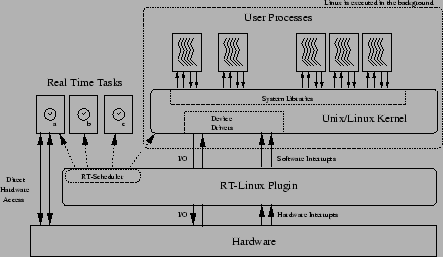
\includegraphics
                                [width=0.7\textwidth]
                                {images/rtlinux_structure.png}
                            \caption
                                [Structure of RTLinux]
                                {Structure of RTLinux \cite{rt-linux-getting-started}.}
                            \label{fig:rtlinux_structure}
                        \end{figure}
                    \item
                        \textbf{Xenomai} works by supplementing the Linux kernel
                            with a real-time kernel running side-by-side with
                            it \cite{xenomai-overview}.
                        The real-time core deals with all time-critical
                            tasks and has a higher priority than the Linux
                            kernel.
                        The Xenomai kernel and the Linux kernel communicate via
                            the
                            \textit{Adaptive Domain Environment for Operating System (ADEOS)},
                            which separate domains for both kernels
                            \cite{preempt-rt-survey}.
                        This is shown in \fig{xenomai_structure}.
                        \begin{figure}[H]
                            \centering
                            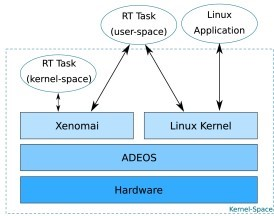
\includegraphics
                                [width=0.5\textwidth]
                                {images/xenomai_structure.jpg}
                            \caption
                                [Structure of Xenomai]
                                {Structure of Xenomai \cite{preempt-rt-survey}.}
                            \label{fig:xenomai_structure}
                        \end{figure}
                    \item
                        \textbf{RTAI} uses a hardware abstraction layer (RTHAL)
                            to get information from Linux and dispatch
                            interrupts \cite{xenomai-overview}.
                        This is displayed in \fig{rtai_structure}.
                        It has few dependencies to Linux, making it easy to
                            switch between versions of the Linux kernel
                            \cite{xenomai-overview}.
                        \begin{figure}[H]
                            \centering
                            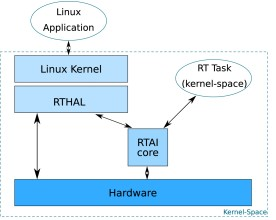
\includegraphics
                                [width=0.5\textwidth]
                                {images/rtai_structure.jpg}
                            \caption
                                [Structure of RTAI]
                                {Structure of RTAI \cite{preempt-rt-survey}.}
                            \label{fig:rtai_structure}
                        \end{figure}
                \end{itemize}

            \subsubsection{Choosing Between the Preemptible Kernel and Real-Time Frameworks}
            % \subsubsection*{Choosing Between Preemptible Kernel and Real-Time Frameworks}
            % \addcontentsline{toc}{subsubsection}{Choosing Between Preemptible Kernel and Real-Time Frameworks}
            % Remove header text
            \markboth{}{}
                The fully preemptible Linux kernel and real-time Linux kernel
                    frameworks both add real-time capabilities to the Linux
                    kernel.
                The fully preemptible kernel achieves this by allowing the
                    kernel to be preempted in kernel mode and utilizing
                    real-time data structures \cite{linux-preemption-models}.
                However, these modifications are not enough to accommodate the
                    needs of a hard real-time system \cite{preempt-rt-survey}.
                At its core, the PREEMPT\_RT patch is still the Linux kernel,
                    offering no guarantees on worst case execution time
                    \cite{preempt-rt-survey}.
                This approach should only be taken for soft real-time systems.
                In this use case, the most important advantage of using the
                    fully preemptible Linux kernel is the cost and speed of
                    development.
                PREEMPT\_RT Linux does not differ much from mainline Linux.
                This allows the wealth of code for drivers and libraries in
                    Linux to be reused---although they may need to be adapted to
                    fit real-time needs.
                Further, many software engineers are competent with Linux and
                    can handle developing with the PREEMPT\_RT patch
                    \cite{preempt-rt-survey}.

                When tighter deadlines are required, a co-kernel Linux framework
                    can be used.
                These frameworks do have the ability to handle hard real-time
                    requirements \cite{preempt-rt-survey}.
                The cost of this functionality is development time and
                    complexity.
                Co-kernel approaches require modifications of the Linux kernel
                    code, none of which are fully backed by the
                    Linux community.
                This also introduces a dependency on the specific Linux kernel
                    version being modified, often being an older version
                    \cite{preempt-rt-survey}.
                The complex interaction between the two kernels introduces a
                    level of complexity that needs to be handled by skilled
                    real-time developers, increasing development efforts
                    \cite{preempt-rt-survey}.
                As a result, real-time Linux frameworks should be used only when
                    necessary, preferring the fully preemptible kernel when
                    timing requirements allow it.

        % Remove header text
        \markboth{}{}
        \subsection{Non-Linux-Based Real Time Operating Systems}
        % \subsection*{Non-Linux-Based Real Time Operating Systems}
        % \addcontentsline{toc}{subsection}{Non-Linux-Based Real Time Operating Systems}
        % Remove header text
        \markboth{}{}
            There are many RTOSs that are not associated with the Linux kernel.
            Some of these operating systems are open source, others are
                commercially available.
            They have different use cases when compared with each other, and
                when compared with Linux-based alternatives.
            These use cases will be presented here, along with examples of
                non-Linux RTOSs.

            \subsubsection{Advantages and Disadvantages of Non-Linux-Based Real-Time Operating Systems}
            % \subsubsection*{Advantages and Disadvantages of Non-Linux-Based Real-Time Operating Systems}
            % \addcontentsline{toc}{subsubsection}{Advantages and Disadvantages of Non-Linux-Based Real-Time Operating Systems}
            % Remove header text
            \markboth{}{}
                The main advantage of using the Linux kernel for real time
                    systems is the ease of development.
                Many software engineers are familiar with Linux and can quickly
                    learn how to use the real-time capabilities of the kernel.
                Soft real-time systems can make use of the fully preemptible
                    kernel, while hard real-time systems require a framework
                    that modifies the kernel.
                However, real-time Linux-based operating systems, whether it is
                    the fully preemptible kernel or a real-time kernel
                    framework, require the memory space and processing power to
                    run a full Linux operating system.
                This is a luxury that many embedded systems simply do not have
                    \cite{rtos-overview}.
                Apart from very large real-time systems, another solution is
                    needed.


    \section{Conclusion}
    % Remove header text
    \markboth{}{}
    % \section*{Conclusion}
    % \addcontentsline{toc}{section}{Conclusion}

    \pagebreak

    % Remove header text
\markboth{}{}

\begin{thebibliography}{99}
\addcontentsline{toc}{section}{References}

    % Remove header text (I don't know why I have to do this twice)
    \markboth{}{}

    \bibitem{textbook}
        A. Silberschatz, P. B. Galvin, G. Gagne,
        \textit{Operating System Concepts}, 10th ed.,
        John Wiley and Sons, Inc., 2018.

    \bibitem{ingelhag}
        J. Ingelhag,
        ``How to choose an operating system for an embedded system'',
        \"Orebro Universitet, 2023.
        Accessed February 9, 2024.
        [Online].
        Available: \urllink{https://www.diva-portal.org/smash/get/diva2:1773441/FULLTEXT01.pdf}.

    \bibitem{whatislinux}
        The Linux Foundation,
        ``What is Linux?,''
        \textit{The Linux Foundation}.
        Accessed February 7, 2024.
        [Online].
        Available: \urllink{https://www.linux.com/what-is-linux/}.

    \bibitem{rtos-overview}
        W. Cede\~no, P.A. Laplante.
        ``An Overview of Real-Time Operating Systems,''
        JALA: Journal of the Association for Laboratory Automation, 2007, ch. 12, sec. 1, pp. 40-45.
        Accessed February 7, 2024.
        [Online].
        Available: \urllink{https://doi.org/10.1016/j.jala.2006.10.016}.

    \bibitem{laplante}
        P. A. Laplante,
        ``Real-Time Systems Design and Analysis,'' 3rd ed.,
        Hoboken, NJ, Wiley, 2004, p. 505.
        Accessed February 7, 2024.
        [Online].
        Available: \urllink{https://doi.org/10.1002/0471648299.fmatter}.

    \bibitem{stallman}
        R. Stallman,
        ``Linux and the GNU System,''
        \textit{Free Software Foundation}.
        Accessed February 9, 2024.
        [Online].
        Available: \urllink{https://www.gnu.org/gnu/linux-and-gnu.en.html}.

    \bibitem{comparative-os}
        A. Adekotujo, A. Odumabo, A. Adedokun, O. Aiyeniko,
        ``A Comparative Study of Operating Systems: Case of Windows, UNIX, Linux, Mac, Android and iOS,''
        International Journal of Computer Applications, 2020.
        Accessed February 10, 2024.
        [Online].
        Available: \href{https://www.researchgate.net/profile/Adedoyin-Odumabo/publication/343013056\_A\_Comparative\_Study\_of\_Operating\_Systems\_Case\_of\_Windows\_UNIX\_Linux\_Mac\_Android\_and\_iOS/links/61f2b50a9a753545e2fe8300/A-Comparative-Study-of-Operating-Systems-Case-of-Windows-UNIX-Linux-Mac-Android-and-iOS.pdf}{https://www.researchgate.net/profile/Adedoyin-Odumabo/publication/343013056\_A\_Comparative\_Study\_of\_Operating\_Systems\_Cas e\_of\_Windows\_UNIX\_Linux\_Mac\_Android\_and\_iOS/links/61f2b50a9a753545e2fe8300 /A-Comparative-Study-of-Operating-Systems-Case-of-Windows-UNIX-Linux-Mac-A ndroid-and-iOS.pdf}.

    \bibitem{grandview}
        Grand View Research,
        ``Server Operating System Market Size, Share \& Trends Analysis Report By Operating System (Windows, Linux), By Virtualization (Virtual Machine, Physical), By Deployment, By Region, And Segment Forecasts, 2022 - 2030,''
        \textit{Grand View Research}, 2020.
        Accessed February 10, 2024.
        [Online].
        Available: \urllink{https://www.grandviewresearch.com/industry-analysis/server-operating-system-market-report}.

    \bibitem{linux-public-cloud}
        The Linux Foundation,
        ``Linux Runs All of the World's Fastest Supercomputers,''
        \textit{The Linux Foundation}, November 20, 2017.
        Accessed February 10, 2024.
        [Online].
        Available: \urllink{https://www.linuxfoundation.org/blog/blog/linux-runs-all-of-the-worlds-fastest-supercomputers}.

    \bibitem{aws-linux}
        L. Clark,
        ``How Amazon Web Services Uses Linux and Open Source,''
        \textit{The Linux Foundation}, September 8, 2014.
        Accessed February 10, 2024.
        [Online].
        Available: \urllink{https://www.linux.com/news/how-amazon-web-services-uses-linux-and-open-source/}.

    \bibitem{bare-metal}
        M. Salehi, D. Hughes, B. Crispo,
        ``MicroGuard: Securing Bare-Metal Microcontrollers against Code-Reuse Attacks,''
        \textit{2019 IEEE Conference on Dependable and Secure Computing (DSC)},
        Hangzhou, China, IEEE, 2019, pp. 1-8, doi: 10.1109/DSC47296.2019.8937667.
        Accessed February 10, 2024.
        [Online].
        Available: \urllink{https://doi.org/10.1109/DSC47296.2019.8937667}.

    \bibitem{embedded-textbook}
        P. Raghavan, A. Lad, S. Neelakandan,
        \textit{Embedded Linux System Design and Development},
        Boca Raton, FL, Taylor and Francis Group, LLC, 2006.

\end{thebibliography}


\end{document}
